
\subsection{Konzeption der Trainingsumgebung} \label{sec:TrainingApproach}
Der \emph{RobotSF} Simulator des Forscherteams aus Triest sieht bereits vor,
zufallsgeneriertes Kartenmaterial mit Hindernissen (Polygone) zu erzeugen und
als JSON-Dateien zu speichern. Wie in Abbildung \ref{fig:MapOld} zu sehen ist, besteht
das Kartenmaterial aus unregelmäßigen, sternförmigen Hindernissen, was mehr einer
Mondlandschaft anstatt einem Gehweg oder einer Fußgänerzone entspricht. Die unrealistischen
Formen von \emph{RobotSF} werden daher durch echtes, aus OpenStreetMap importiertes
Kartenmaterial ersetzt und mithilfe des \emph{Map Editors} aufbereitet. Dies erfordert
eine Effizienzoptimierung der Simulationsumgebung, auf die im darauffolgenden Abschnitt
\ref{sec:SimEffOpt} eingegangen wird.

\begin{figure}[h]
  \centering
  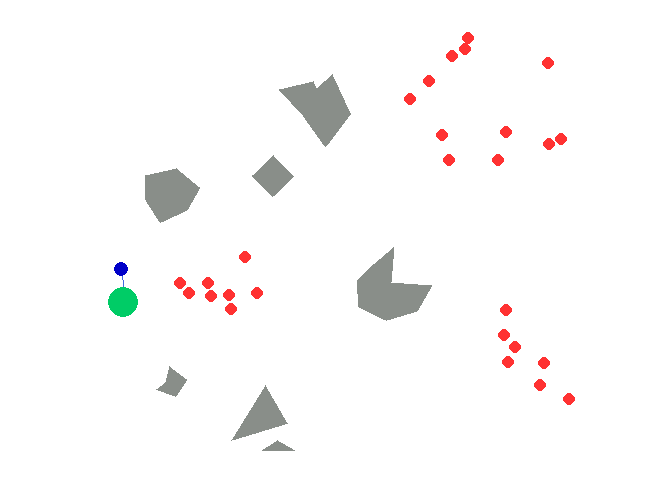
\includegraphics[width = 0.65\textwidth]{imgs/kartenmaterial_alt}
  \caption{Beispiel für altes Kartenmaterial des \emph{RobotSF} Simulators}
  \label{fig:MapOld}
\end{figure}

Als Kartenmaterial für die Trainingsumgebungen werden zwei echte Karten gewählt. Wie in
Abbildung \ref{fig:Scenario_1} zu sehen ist, besteht die erste Trainingsumgebung aus
einigen miteinander verbundenen Häuserblocks nahe des Universitätsgeländes, in deren
Innenhöfen künstliche, in orange dargestellte Fußgängerzonen angelegt werden, um belebte
Plätze zu simulieren. Das Fahrzeug startet in der blau markierten Zone und folgt den
durch die grünen Punkte dargestellten Routen bis hin zur jeweiligen Zielzone. Die Routen
verlaufen in alle Himmelsrichtungen und führen bewusst durch mindestens eine Menschenmenge.\\

\begin{figure}[h]
  \centering
  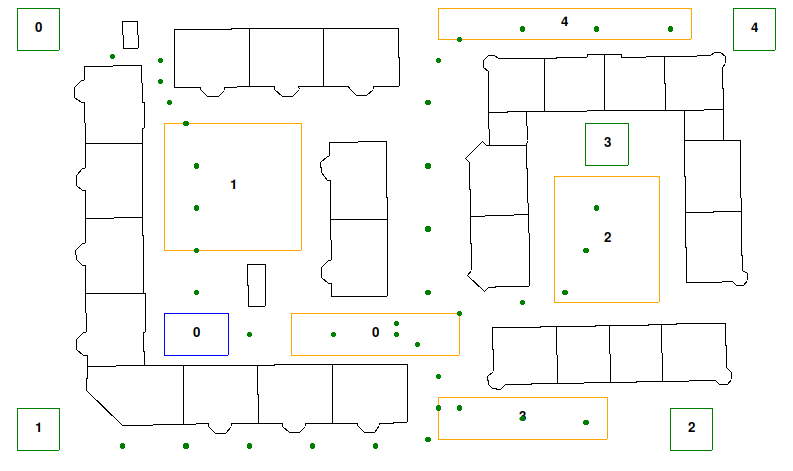
\includegraphics[width = 1.0\textwidth]{imgs/small_map}
  \caption{Erste Trainingsumgebung des überarbeiteten \emph{RobotSF} Simulators}
  \label{fig:Scenario_1}
\end{figure}

Dadurch dass der Agent gezwungen wird, durch Menschenmengen zu fahren, soll die sichere
Interaktion mit Fußgängern erlernt werden. Die Verkehrsdichte in den orange markierten
Fußgängerzonen kann während der Trainingsläufe und Evaluationen variiert werden, um die
Robustheit der erlernten Fahrverhaltensweise zu prüfen. Durch das Ein- und Ausschalten
der \emph{Ped-Robot Force} wird das Verhalten der Fußgänger dahingehend modifiziert,
ob sie das Fahrzeug wahrnehmen können und ihm ausweichen. Durch die Modifikation des
Fußgängerverhaltens bezüglich der Wahrnehmung des Fahrzeugs während des Trainings soll
gesteuert werden, ob der Agent offensiveres oder defensiveres Fahrverhalten lernt.\\

Für die zweite Trainingsumgebung wird eine Karte des Campus der Universität Augsburg
gewählt, da sich entsprechendes Kartenmaterial als verkehrsberuhigter Bereich mit viel
Fußgängerverkehr bestens für die virtuelle Erprobung autonomer Mikromobilitätsahrzeuge
anbietet und auch perspektivisch die Evaluationen echter Fahrzeuge in der Realität ermöglicht.
Wie in Abbildung \ref{fig:Scenario_2} zu sehen, umfassen die in grün dargestellten Start- und
Zielorte des Fahrzeugs das Unikum (0), das Rote Pferd (1), die Alte Cafeteria (2),
den Durchgang zwischen N-Gebäude und Mensa (3), das Prüfungsamt (4), den Ausgang zum
Messeparkplatz (5), die Juristische Fakultät (6), den Eingang zur Wirtschaftsinformatik (7),
den Eingang zum C-Hörsaal (8), den Eingang zur Zentralbibliothek (9) und den Eingang zur
mathematisch-naturwissenschaftlichen Bibliothek (10).
Am Wasserspiel (0, 1), vor der Zentralbibliothek (2), vor der Brücke (3) und bei den
Straßenbahnhaltestellen (4, 5) befinden sich die orange markierten Fußgängerzonen, um dichten
Verkehr zu simulieren. Zudem verlaufen auf allen befahrenen Gehwegen die mit gelben Punkten
dargestellten Fußgängerrouten in beide Laufrichtungen, um typischen Verkehr zu generieren.\\

\begin{figure}[h]
  \centering
  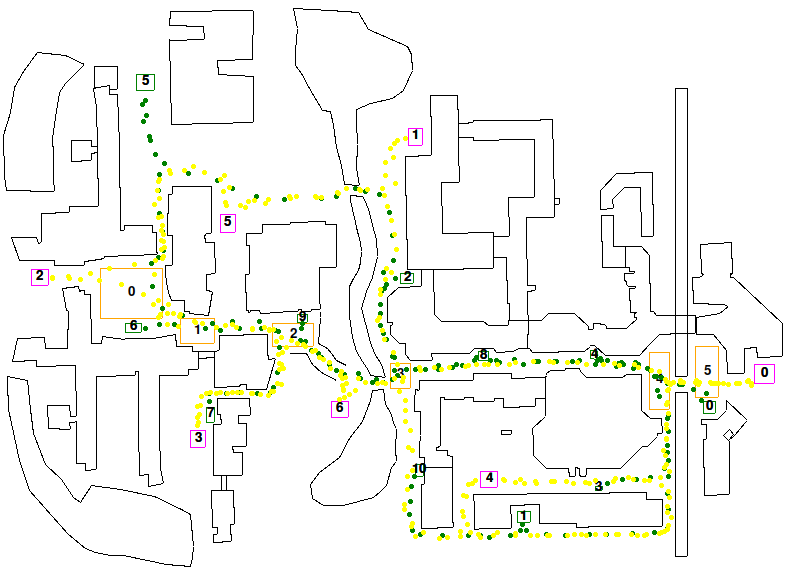
\includegraphics[width = 1.0\textwidth]{imgs/campus_map}
  \caption{Zweite Trainingsumgebung des überarbeiteten \emph{RobotSF} Simulators.
  Das Kartenmaterial zeigt den Campus der Universität Augsburg.}
  \label{fig:Scenario_2}
\end{figure}

Das Design der Routen sieht vor, verschiedenste Situationen herbeizuführen, die auch
in der Realität auftreten können. Auf den Gehwegen wird hauptsächlich getestet,
ob der Agent die Bewegung der Fußgänger korrekt einschätzen und Überholmanöver
in engen Räumen sicher durchführen kann. Nah an Hauswänden verlaufende 90-Grad Kurven
prüfen, ob vor der Kurve abgebremst wird, da der Agent nur eine eingeschränkte Sicht
auf den sich hinter der Wand befindlichen Gegenverkehr hat. Hingegen wird auf großen,
belebten Plätzen wie bereits bei der ersten Trainingsumgebung die Fähigkeit zur
Kollisionsvermeidung und Erzielung von Fortschritten in dichten Menschenmengen getestet.
Dabei soll der Agent ein möglichst defensives Verhalten aufweisen, damit sich die Fußgänger
sicher fühlen können. Durch Engstellen soll der Agent lernen, erst zu fahren, sobald eine
befahrbare Passage frei wird. Dies erfordert unter anderem eine Einschätzung, ob die
Engstelle lange genug befahrbar bleibt, um sie zu passieren.
